

\documentclass[letterpaper,hide notes,xcolor={table,svgnames},pdftex,10pt]{beamer}
\def\showexamples{t}


%\usepackage[svgnames]{xcolor}

%% Demo talk
%\documentclass[letterpaper,notes=show]{beamer}

\usecolortheme{crane}
\setbeamertemplate{navigation symbols}{}

\usetheme{MyPittsburgh}
%\usetheme{Frankfurt}

%\usepackage{tipa}

\usepackage{hyperref}
\usepackage{graphicx,xspace}
\usepackage[normalem]{ulem}
\usepackage{multicol}
\usepackage{amsmath,amssymb,amsthm,graphicx,xspace}
\newcommand\SF[1]{$\bigstar$\footnote{SF: #1}}

\usepackage[default]{sourcesanspro}
\usepackage[T1]{fontenc}
\usepackage[scaled]{beramono}
\usepackage{tikzpagenodes}

\newcounter{tmpnumSlide}
\newcounter{tmpnumNote}


% old question code
%\newcommand\question[1]{{$\bigstar$ \small \onlySlide{2}{#1}}}
% \newcommand\nquestion[1]{\ifdefined \presentationonly \textcircled{?} \fi \note{\par{\Large \textbf{?}} #1}}
% \newcommand\nanswer[1]{\note{\par{\Large \textbf{A}} #1}}


 \newcommand\mnote[1]{%
   \addtocounter{tmpnumSlide}{1}
   \ifdefined\showcues {~\tiny\fbox{\arabic{tmpnumSlide}}}\fi
   \note{\setlength{\parskip}{1ex}\addtocounter{tmpnumNote}{1}\textbf{\Large \arabic{tmpnumNote}:} {#1\par}}}

\newcommand\mmnote[1]{\note{\setlength{\parskip}{1ex}#1\par}}

%\newcommand\mnote[2][]{\ifdefined\handoutwithnotes {~\tiny\fbox{#1}}\fi
% \note{\setlength{\parskip}{1ex}\textbf{\Large #1:} #2\par}}

%\newcommand\mnote[2][]{{\tiny\fbox{#1}} \note{\setlength{\parskip}{1ex}\textbf{\Large #1:} #2\par}}

\newcommand\mquestion[2]{{~\color{red}\fbox{?}}\note{\setlength{\parskip}{1ex}\par{\Large \textbf{?}} #1} \note{\setlength{\parskip}{1ex}\par{\Large \textbf{A}} #2\par}\ifdefined \presentationonly \pause \fi}

\newcommand\blackboard[1]{%
\ifdefined   \showblackboard
  {#1}
  \else {\begin{center} \fbox{\colorbox{blue!30}{%
         \begin{minipage}{.95\linewidth}%
           \hspace{\stretch{1}} Some space intentionally left blank; done at the blackboard.%
         \end{minipage}}}\end{center}}%
         \fi%
}



%\newcommand\q{\tikz \node[thick,color=black,shape=circle]{?};}
%\newcommand\q{\ifdefined \presentationonly \textcircled{?} \fi}

\usepackage{listings}
\lstset{basicstyle=\footnotesize\ttfamily,
	breaklines=true,
	aboveskip=15pt,
  	belowskip=15pt,
	frame=lines,
	numbers=left, basicstyle=\scriptsize, numberstyle=\tiny, stepnumber=0, numbersep=2pt
}

\usepackage{siunitx}
\newcommand\sius[1]{\num[group-separator = {,}]{#1}\si{\micro\second}}
\newcommand\sims[1]{\num[group-separator = {,}]{#1}\si{\milli\second}}
\newcommand\sins[1]{\num[group-separator = {,}]{#1}\si{\nano\second}}
\sisetup{group-separator = {,}, group-digits = true}

%% -------------------- tikz --------------------
\usepackage{tikz}
\usetikzlibrary{positioning}
\usetikzlibrary{arrows,backgrounds,automata,decorations.shapes,decorations.pathmorphing,decorations.markings,decorations.text,decorations.pathreplacing}

\tikzstyle{place}=[circle,draw=blue!50,fill=blue!20,thick, inner sep=0pt,minimum size=6mm]
\tikzstyle{transition}=[rectangle,draw=black!50,fill=black!20,thick, inner sep=0pt,minimum size=4mm]

\tikzstyle{block}=[rectangle,draw=black, thick, inner sep=5pt]
\tikzstyle{bullet}=[circle,draw=black, fill=black, thin, inner sep=2pt]

\tikzstyle{pre}=[<-,shorten <=1pt,>=stealth',semithick]
\tikzstyle{post}=[->,shorten >=1pt,>=stealth',semithick]
\tikzstyle{bi}=[<->,shorten >=1pt,shorten <=1pt, >=stealth',semithick]

\tikzstyle{mut}=[-,>=stealth',semithick]

\tikzstyle{treereset}=[dashed,->, shorten >=1pt,>=stealth',thin]

\usepackage{ifmtarg}
\usepackage{xifthen}
\makeatletter
% new counter to now which frame it is within the sequence
\newcounter{multiframecounter}
% initialize buffer for previously used frame title
\gdef\lastframetitle{\textit{undefined}}
% new environment for a multi-frame
\newenvironment{multiframe}[1][]{%
\ifthenelse{\isempty{#1}}{%
% if no frame title was set via optional parameter,
% only increase sequence counter by 1
\addtocounter{multiframecounter}{1}%
}{%
% new frame title has been provided, thus
% reset sequence counter to 1 and buffer frame title for later use
\setcounter{multiframecounter}{1}%
\gdef\lastframetitle{#1}%
}%
% start conventional frame environment and
% automatically set frame title followed by sequence counter
\begin{frame}%
\frametitle{\lastframetitle~{\normalfont(\arabic{multiframecounter})}}%
}{%
\end{frame}%
}
\makeatother

\makeatletter
\newdimen\tu@tmpa%
\newdimen\ydiffl%
\newdimen\xdiffl%
\newcommand\ydiff[2]{%
    \coordinate (tmpnamea) at (#1);%
    \coordinate (tmpnameb) at (#2);%
    \pgfextracty{\tu@tmpa}{\pgfpointanchor{tmpnamea}{center}}%
    \pgfextracty{\ydiffl}{\pgfpointanchor{tmpnameb}{center}}%
    \advance\ydiffl by -\tu@tmpa%
}
\newcommand\xdiff[2]{%
    \coordinate (tmpnamea) at (#1);%
    \coordinate (tmpnameb) at (#2);%
    \pgfextractx{\tu@tmpa}{\pgfpointanchor{tmpnamea}{center}}%
    \pgfextractx{\xdiffl}{\pgfpointanchor{tmpnameb}{center}}%
    \advance\xdiffl by -\tu@tmpa%
}
\makeatother
\newcommand{\copyrightbox}[3][r]{%
\begin{tikzpicture}%
\node[inner sep=0pt,minimum size=2em](ciimage){#2};
\usefont{OT1}{phv}{n}{n}\fontsize{4}{4}\selectfont
\ydiff{ciimage.south}{ciimage.north}
\xdiff{ciimage.west}{ciimage.east}
\ifthenelse{\equal{#1}{r}}{%
\node[inner sep=0pt,right=1ex of ciimage.south east,anchor=north west,rotate=90]%
{\raggedleft\color{black!50}\parbox{\the\ydiffl}{\raggedright{}#3}};%
}{%
\ifthenelse{\equal{#1}{l}}{%
\node[inner sep=0pt,right=1ex of ciimage.south west,anchor=south west,rotate=90]%
{\raggedleft\color{black!50}\parbox{\the\ydiffl}{\raggedright{}#3}};%
}{%
\node[inner sep=0pt,below=1ex of ciimage.south west,anchor=north west]%
{\raggedleft\color{black!50}\parbox{\the\xdiffl}{\raggedright{}#3}};%
}
}
\end{tikzpicture}
}


%% --------------------

%\usepackage[excludeor]{everyhook}
%\PushPreHook{par}{\setbox0=\lastbox\llap{MUH}}\box0}

%\vspace*{\stretch{1}

%\setbox0=\lastbox \llap{\textbullet\enskip}\box0}

\setlength{\parskip}{\fill}

\newcommand\noskips{\setlength{\parskip}{1ex}}
\newcommand\doskips{\setlength{\parskip}{\fill}}

\newcommand\xx{\par\vspace*{\stretch{1}}\par}
\newcommand\xxs{\par\vspace*{2ex}\par}
\newcommand\tuple[1]{\langle #1 \rangle}
\newcommand\code[1]{{\sf \footnotesize #1}}
\newcommand\ex[1]{\uline{Example:} \ifdefined \presentationonly \pause \fi
  \ifdefined\showexamples#1\xspace\else{\uline{\hspace*{2cm}}}\fi}

\newcommand\ceil[1]{\lceil #1 \rceil}


\AtBeginSection[]
{
   \begin{frame}
       \frametitle{Outline}
       \tableofcontents[currentsection]
   \end{frame}
}



\pgfdeclarelayer{edgelayer}
\pgfdeclarelayer{nodelayer}
\pgfsetlayers{edgelayer,nodelayer,main}

\tikzstyle{none}=[inner sep=0pt]
\tikzstyle{rn}=[circle,fill=Red,draw=Black,line width=0.8 pt]
\tikzstyle{gn}=[circle,fill=Lime,draw=Black,line width=0.8 pt]
\tikzstyle{yn}=[circle,fill=Yellow,draw=Black,line width=0.8 pt]
\tikzstyle{empty}=[circle,fill=White,draw=Black]
\tikzstyle{bw} = [rectangle, draw, fill=blue!20, 
    text width=4em, text centered, rounded corners, minimum height=2em]
    
    \newcommand{\CcNote}[1]{% longname
	This work is licensed under the \textit{Creative Commons #1 3.0 License}.%
}
\newcommand{\CcImageBy}[1]{%
	\includegraphics[scale=#1]{creative_commons/cc_by_30.pdf}%
}
\newcommand{\CcImageSa}[1]{%
	\includegraphics[scale=#1]{creative_commons/cc_sa_30.pdf}%
}
\newcommand{\CcImageNc}[1]{%
	\includegraphics[scale=#1]{creative_commons/cc_nc_30.pdf}%
}
\newcommand{\CcGroupBySa}[2]{% zoom, gap
	\CcImageBy{#1}\hspace*{#2}\CcImageNc{#1}\hspace*{#2}\CcImageSa{#1}%
}
\newcommand{\CcLongnameByNcSa}{Attribution-NonCommercial-ShareAlike}

\newenvironment{changemargin}[1]{% 
  \begin{list}{}{% 
    \setlength{\topsep}{0pt}% 
    \setlength{\leftmargin}{#1}% 
    \setlength{\rightmargin}{1em}
    \setlength{\listparindent}{\parindent}% 
    \setlength{\itemindent}{\parindent}% 
    \setlength{\parsep}{\parskip}% 
  }% 
  \item[]}{\end{list}} 




\title{Lecture 15 --- Rate Limits}

\author{Jeff Zarnett\\ \small \texttt{jzarnett@uwaterloo.ca}}
\institute{Department of Electrical and Computer Engineering \\
  University of Waterloo}
\date{\today}


\begin{document}

\begin{frame}
  \titlepage
 \end{frame}
 
\begin{frame}
\frametitle{It's Not Me, It's You}

\begin{center}
  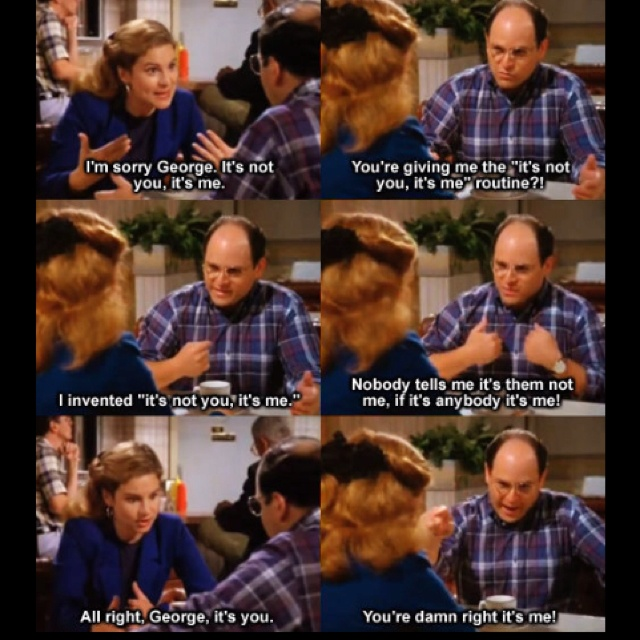
\includegraphics[width=0.7\textwidth]{images/its-me.jpg}
\end{center}

\end{frame}

\begin{frame}
\frametitle{Speed Limit}

\begin{center}
  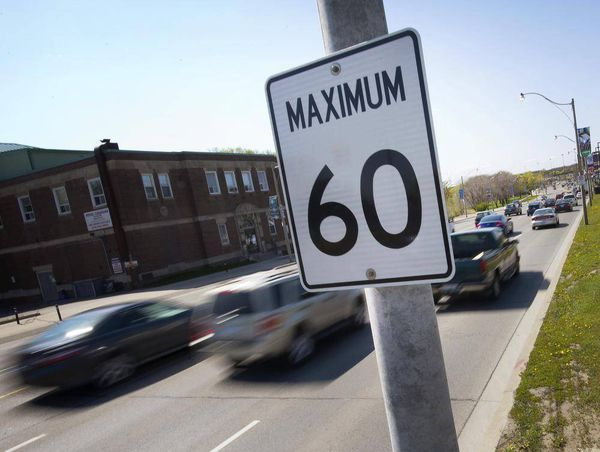
\includegraphics[width=0.4\textwidth]{images/speedlimit.jpg}
\end{center}

Sometimes the limiting factor in an app is not under our control.

A rate limit is exactly what it sounds like.

\end{frame}

\begin{frame}
\frametitle{More Complex}

Rate limits can be more complicated than just requests per unit time. 

Multiple thresholds (e.g., A requests per hour or B requests per day)?

Max C requests to change your user data per day, and a max of D requests of any type per day in total?

Slow down vs just reject? We'll just reject for now.

\end{frame}

\begin{frame}
\frametitle{Rejection Hurts}

Rejected requests can be a huge problem for your application or service.

Obvious example: using ChatGPT in your app?

Other example: validating webhooks that the service itself sent in...

\end{frame}

\begin{frame}
\frametitle{Why Are Limits?}

\begin{center}
  
\includegraphics[width=0.5\textwidth]{images/its-the-law.jpg}
\end{center}

Rate limits exist because every request has a certain cost associated with it.

The cost may or may not be measured in currency.

Consider opportunity cost.

\end{frame}

\begin{frame}
\frametitle{DoS and DDoS}
\alert{Denial of Service (DoS)} attack: negatively impact some service by submitting many invalid requests to overwhelm it.

\begin{center}
  
\includegraphics[width=0.5\textwidth]{images/bombardment.jpg}
\end{center}

If using numerous clients: \alert{Distributed Denial of Service (DDoS)} attack. 

\end{frame}

\begin{frame}
\frametitle{Rate Limit Example}

Using a system that allowed Ontarians to write letters to the Minister of the Environment about allowing rock climbing in provincial parks. 

We were encouraging people at climbing gyms to send letters (well, emails).

The climbing gym IP address got rate limited because people were sending letters from the gym's wifi.

\end{frame}

\begin{frame}
\frametitle{Request Consume Resources}

Consider the Unity Engine's proposed (retracted) changes in 2023.

Charge per installation? What if I write an install bomb?

\begin{center}
  
\includegraphics[width=0.5\textwidth]{images/unityengine.jpg}
\end{center}

\end{frame}

\begin{frame}
\frametitle{Scraping All Data}

Rate limits can also prevent scraping all your data.

This really happened to the openly-political social media site ``Parler''.

Two bad decisions: sequential post IDs and no rate limits.

\end{frame}

\begin{frame}
\frametitle{For Whose Benefit?}

Concern: if others can scrape all your content for their own benefit at your cost.

Even if it's intended as non-malicious training some machine learning model. 

\begin{center}
  
\includegraphics[width=0.3\textwidth]{images/openaitraining.jpg}
\end{center}

Yes, OpenAI did scan the internet to train ChatGPT.

\end{frame}

\begin{frame}
\frametitle{Dealing with Rate Limits}

Assume we have a system with a rate limit and we need to address that.

If the rate limit is super high compared to usage, no problem.

Hitting the rate limit regularly? Frustrating or could get us banned!

\end{frame}

\begin{frame}
\frametitle{What's the Limit?}
If we get rejected requests we know there's a problem, but what's the limit?

\begin{itemize}
	\item Does the documentation tell us?
	\item Is there an API to query it?
	\item Does it come in the responses?
	\item None of the above?
\end{itemize}

Why not tell us?

\end{frame}


\begin{frame}
\frametitle{Atlassian Makes No Promises}

\textit{``REST API rate limits are not published because the computation logic is evolving continuously to maximize reliability and performance for customers'' }

It does give them more freedom?

Testing for the limit here might work but information is out-of-date quickly.

\end{frame}

\begin{frame}
\frametitle{What Can We Do?}

Giving up: not the right answer... especially in an interview.

Can we do less work? Might help, but how much redundancy will we find?

\end{frame}

\begin{frame}
\frametitle{Caching}

Remember answers previously received. 

Remember what we discussed about write-through and write-back caches.

It can be difficult to know if the data is changed remotely.\\
\quad Use domain knowledge here! e.g., exchange rate quotes valid 20 mins.

\end{frame}

\begin{frame}
\frametitle{Group Up}

Can we group up requests into a larger one?

\begin{center}
  
\includegraphics[width=0.6\textwidth]{images/assemble.jpg}
\end{center}

There do need to be things to group with...

And perhaps the remote API has to support it.

\end{frame}

\begin{frame}
\frametitle{Bigger Requests, Bigger Parsing}

Grouping requests may also make it hard to handle what happens if there's a problem with one of the elements in it. 

If we asked to update five employees and one of the requests is invalid, is the whole group rejected or just the one employee update?

Consider the risks of more complex logic.

\end{frame}

\begin{frame}
\frametitle{Patience}

\begin{center}
  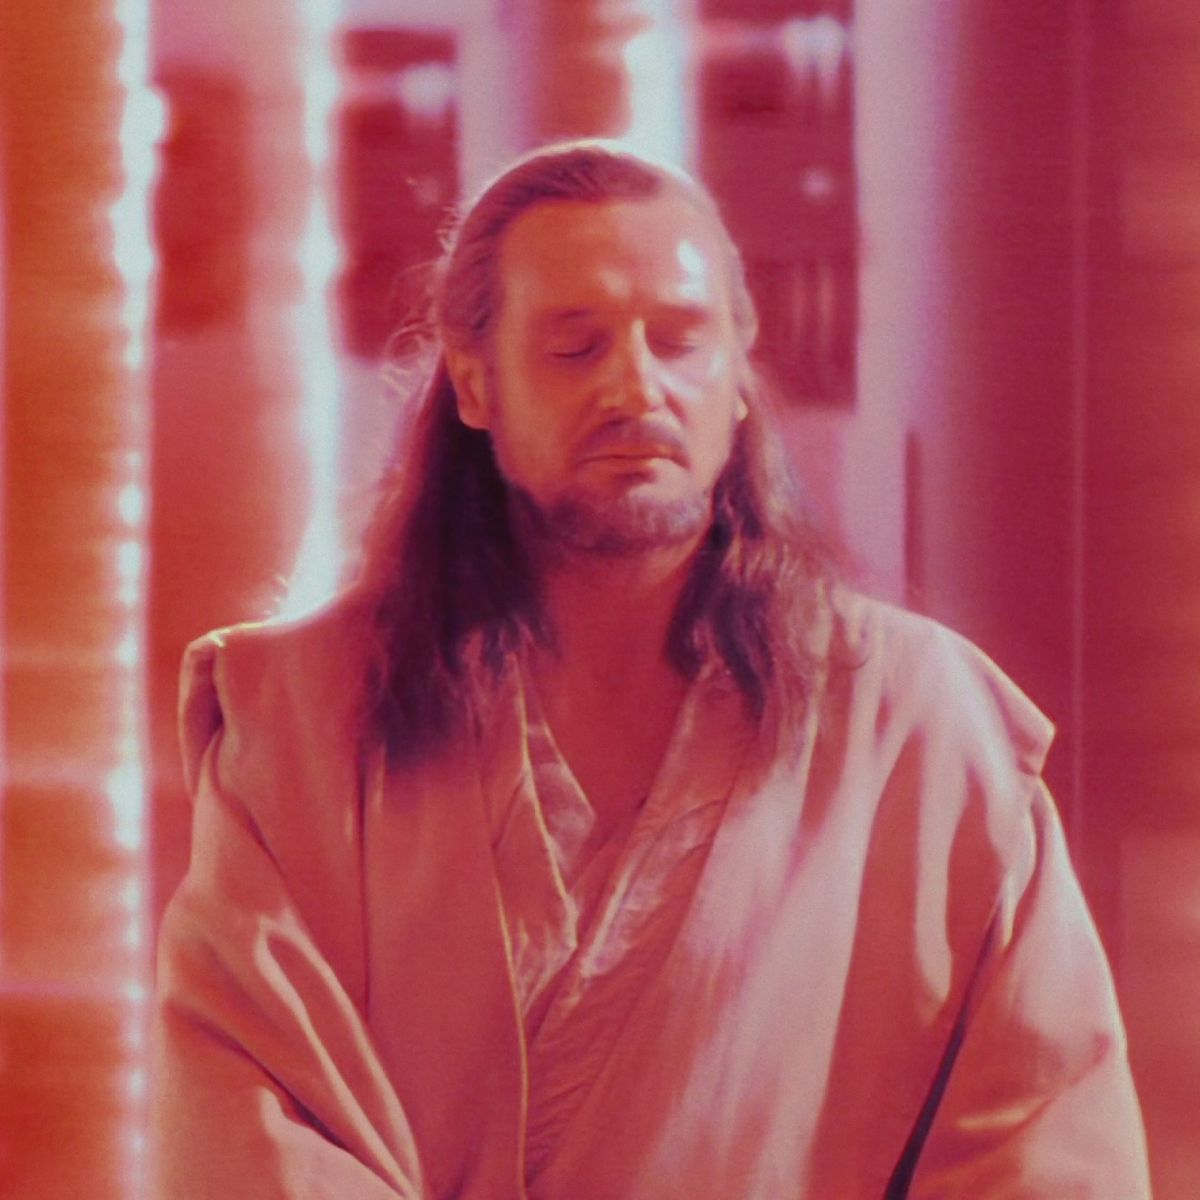
\includegraphics[width=0.4\textwidth]{images/patience.jpg}
\end{center}

If the problem is that too many requests are happening in a short period of time, maybe our best solution is to distribute the requests over more time.

\end{frame}

\begin{frame}
\frametitle{Patience}
When there is a more demand for something than capacity, what do we do?

\begin{center}
  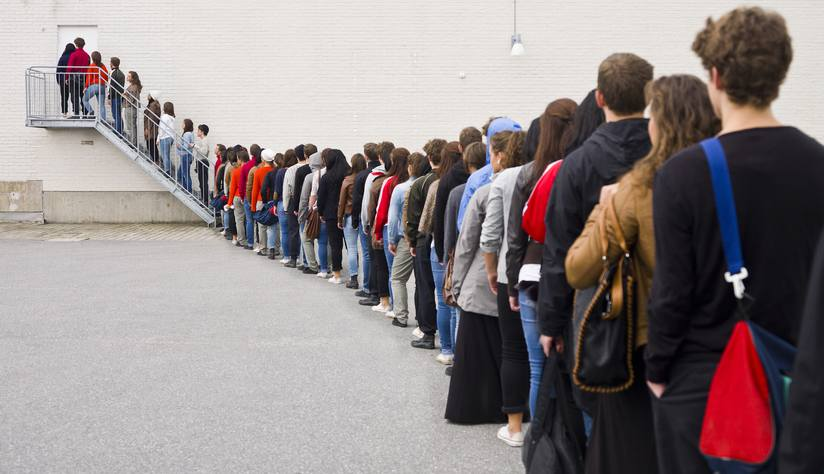
\includegraphics[width=0.7\textwidth]{images/lineup.jpg}
\end{center}

Simply controlling the rate at which requests leave the queue is sufficient to ensure that the rate limit is not exceeded. 

\end{frame}

\begin{frame}
\frametitle{Rust Crates}

Unsurprisingly, multiple Rust crates do what we want. 

Below are some examples from the documentation of the \texttt{ratelimit} crate.

This is not especially fancy, but is sufficient for an example.

\end{frame}

\begin{frame}[fragile]
\frametitle{Rust Rate Limit}
\begin{lstlisting}[language=Rust]
use ratelimit::Ratelimiter;
use std::time::Duration;

// Constructs a ratelimiter that generates 1 tokens/s with no burst. This
// can be used to produce a steady rate of requests. The ratelimiter starts
// with no tokens available, which means across application restarts, we
// cannot exceed the configured ratelimit.
let ratelimiter = Ratelimiter::builder(1, Duration::from_secs(1))
    .build()
    .unwrap();

// Another use case might be admission control, where we start with some
// initial budget and replenish it periodically. In this example, our
// ratelimiter allows 1000 tokens/hour. For every hour long sliding window,
// no more than 1000 tokens can be acquired. But all tokens can be used in
// a single burst. Additional calls to `try_wait()` will return an error
// until the next token addition.
//
// This is popular approach with public API ratelimits.
let ratelimiter = Ratelimiter::builder(1000, Duration::from_secs(3600))
    .max_tokens(1000)
    .initial_available(1000)
    .build()
    .unwrap();
\end{lstlisting}

\end{frame}

\begin{frame}[fragile]
\frametitle{Rust Rate Limit}
\begin{lstlisting}[language=Rust]
// For very high rates, we should avoid using too short of an interval due
// to limits of system clock resolution. Instead, it's better to allow some
// burst and add multiple tokens per interval. The resulting ratelimiter
// here generates 50 million tokens/s and allows no more than 50 tokens to
// be acquired in any 1 microsecond long window.
let ratelimiter = Ratelimiter::builder(50, Duration::from_micros(1))
    .max_tokens(50)
    .build()
    .unwrap();

// constructs a ratelimiter that generates 100 tokens/s with no burst
let ratelimiter = Ratelimiter::builder(1, Duration::from_millis(10))
    .build()
    .unwrap();

for _ in 0..10 {
    // a simple sleep-wait
    if let Err(sleep) = ratelimiter.try_wait() {
           std::thread::sleep(sleep);
           continue;
    }
    // do some ratelimited action here    
}
\end{lstlisting}
\end{frame}

\begin{frame}
\frametitle{Users Are Impatient}

Enqueueing a request is not always suitable if the user is sitting at the screen and awaiting a response to their request.

It takes a synchronous flow and makes it asynchronous.

Rearchitecting it can be a long-term goal, or just something we do with requests that don't have to be synchronous to make room.

\end{frame}

\begin{frame}
\frametitle{Schedule Later}

For requests that are not urgent, then another option is to schedule the requests for a not-busy time.

\begin{center}
  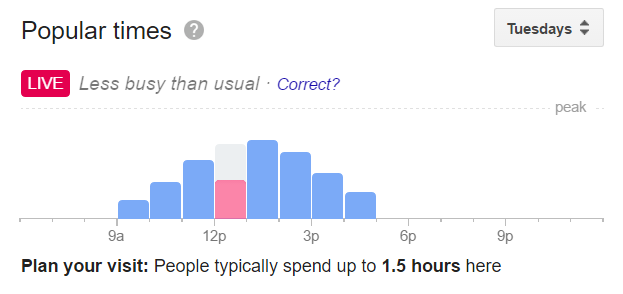
\includegraphics[width=0.7\textwidth]{images/popular-times.png}
\end{center}

Overnight might be a great time to do things that count against the limit.

\end{frame}

\begin{frame}
\frametitle{Billing Examples}

Imagine that you have a billing system where the monthly invoicing procedure uses the majority of the rate limit. 

If that happens during the day, then there's no capacity for adding new customers, updating them, paying invoices, etc. 

The solution then is to run the invoicing procedure overnight instead.

\end{frame}

\begin{frame}
\frametitle{Billing Examples}

Maybe you can even convince management to make it so not all users are billed on the first of the month, but that might require some charisma.


Which leads us to the next idea\ldots

\end{frame}

\begin{frame}
\frametitle{Roll Persuasion}

Convince the other side to raise the limit?

\begin{center}
  
\includegraphics[width=0.4\textwidth]{images/certainly-try.jpg}
\end{center}

Sometimes it's negotiated, sometimes you need to pay more money, sometimes it's just not possible.

\end{frame}

\begin{frame}
\frametitle{It Happened Anyway}

We might still encounter the occasional rate limit. 

That's not a disaster, as long as we handle it the right way. 

The right way is not try harder or try more; if we are being rate limited then we need to try again later, but how much later?

\end{frame}

\begin{frame}
\frametitle{The Answer is Right There}

Sometimes the answer for how long to wait is in the API response.

\begin{center}
  
\includegraphics[width=0.4\textwidth]{images/khaby.png}
\end{center}

... if we read it.

\end{frame}

\begin{frame}
\frametitle{Exponential Backoff}


\begin{center}
	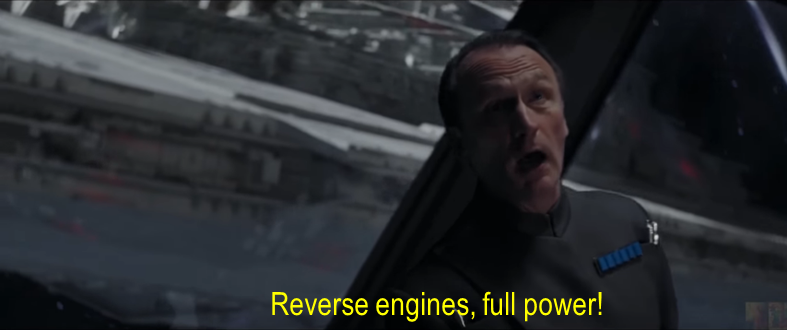
\includegraphics[width=0.7\textwidth]{images/reverse.png}
\end{center}

Resources might not be available right now; retry later?

It's unhelpful to have a tight loop that simply retries as fast as possible. 

Wait a little bit and try again; if the error occurs, next time wait a little longer.

\end{frame}

\begin{frame}
\frametitle{Press F5 Until the Website Loads!}

Repeatedly retrying doesn't help. 

If it's down for maintenance, it could be quite a while before it's back.

Or, if the resource is overloaded right now, the reaction of requesting it more will make it even more overloaded and makes the problem worse! 


\end{frame}

\begin{frame}
\frametitle{Jitter}


The exponential backoff with jitter strategy is good for a scenario where you have lots of independent clients accessing the same resource.

If you have one client, maybe you want something like TCP congestion control.

\end{frame}





\end{document}

